\documentclass[UTF8]{ctexart}
\usepackage{graphicx}
\usepackage{float}
\usepackage{url}
\usepackage{geometry}
\usepackage{fancyhdr}
\usepackage{lastpage}
\usepackage{amsmath}
\usepackage{booktabs}
\usepackage{multicol}
\usepackage{multirow}
\usepackage{color}
\usepackage{subfigure}
\usepackage{listings}
\geometry{left=2.54cm,right=2.54cm,top=3.18cm,bottom=3.18cm}%页边距
\pagestyle{fancy}
\lhead{
\includegraphics[scale=1]{sjtu-logo-red.pdf}}  
\rhead{mini-PACS系统的搭建} 
\cfoot{第 \thepage\ 页\ 共 \pageref{LastPage} 页}   

\lstset{
    basicstyle          =   \sffamily,          % 基本代码风格
    keywordstyle        =   \bfseries\color{blue},          % 关键字风格
    commentstyle        =   \rmfamily\itshape,  % 注释的风格,斜体
    stringstyle         =   \ttfamily,  % 字符串风格
    flexiblecolumns,                % 别问为什么,加上这个
    numbers             =   left,   % 行号的位置在左边
    showspaces          =   false,  % 是否显示空格,显示了有点乱,所以不现实了
    numberstyle         =   \zihao{-5}\ttfamily,    % 行号的样式,小五号,tt等宽字体
    showstringspaces    =   false,
    captionpos          =   t,      % 这段代码的名字所呈现的位置,t指的是top上面
    frame               =   lrtb,   % 显示边框
}

\begin{document}
\bibliographystyle{unsrt}
\begin{titlepage}
    \begin{center}
        
\includegraphics[width=0.8\textwidth]{sjtu-name-blue.pdf}\\[1cm]
        \textsc{\Huge \bfseries 课程报告}\\[1.5cm]
        
\includegraphics[width=0.3\textwidth]{sjtu-badge-blue.pdf}\\[0.5cm]

        \Huge \bfseries{mini-PACS系统的搭建}\\[1cm]
        \Large \bfseries{518021910971 裴奕博}
    \end{center}
\end{titlepage}
\tableofcontents
\newpage

\begin{abstract}
    本报告详细叙述了一个mini-PACS系统的搭建流程,从开源软件的选择到搭建和功能的调试和log的解析,以及在搭建过程中遇到的各种问题。
    \textbf{关键字:} 开源软件,mini-PACS,Orthanc,DCMTK
\end{abstract}
%正文
\section{开源软件的选择}
\subsection{Server和SCP的选择}
在上次的开源软件调研报告中,我了解到了几个目前流行的开源mini-PACS框架,其中就有Orthanc。Orthanc是一个基于C++开发的轻量级mini-PACS框架,采用GPL协议开源。它具有以下几个特点\cite{enwiki:1041672725}:
\begin{enumerate}
    \item 提供了内置的http服务,可以通过Web应用来可视化的上传、查看、检索和传输Dicom文件。
    \item 跨平台。可以在Windows下运行,也可以通过Docker在Linux下运行,可以部署在常见的网站服务器上如Nginx、Apache等。
    \item 可以通过多种方式实现Dicom的传输。不仅提供了Dicom Server端口,也可以使用Web应用可视化上传,更是提供了REST API直接上传Dicom文件。
\end{enumerate}
\begin{figure}[H]
    \centering
    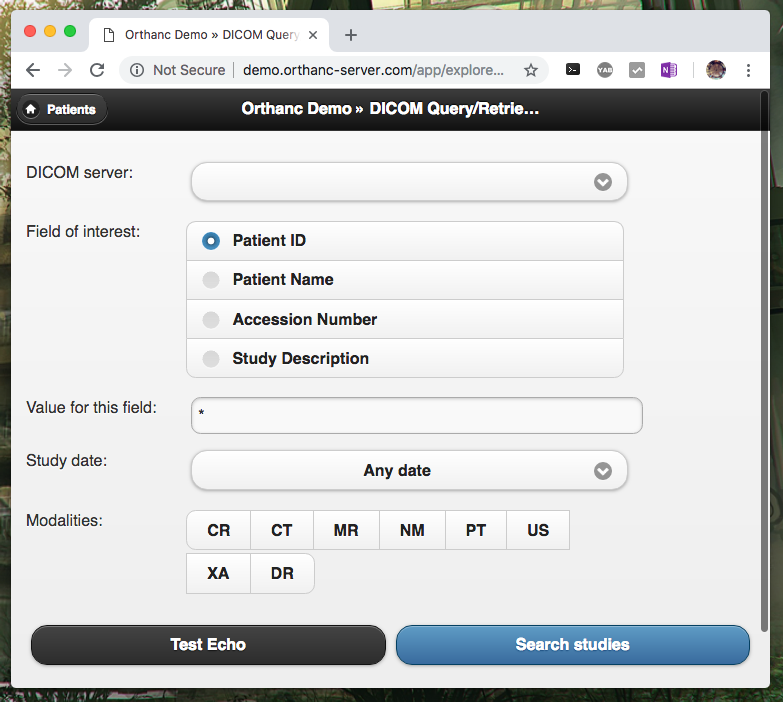
\includegraphics[width=0.4\textwidth]{orthanc.png}
    \caption{Orthanc界面}
    \label{fig:Orthanc}
\end{figure}

Orthanc目前仍然在持续更新中,更加现代化,界面也漂亮舒适。因此在本次实验中选择了Orthanc作为Dicom Server和SCP。其中,Server运行在windows本地,SCP运行在WSL的Docker下。

\subsection{SCU的选择}
由于Orthanc提供了多种传输方式,因此此次实验既尝试使用了开源的DCMTK作为SCU,也尝试了直接使用Web应用上传。

DCMTK是由德国offis公司提供的开源项目,使用C++实现了Dicom协议的相关细节,并封装成了各个应用,为我们提供了实现DICOM协议的一个平台,使得我们可以在它的基础上轻松的完成自己的主要工作,而不必把太多的精力放在实现DICOM协议的细节问题上\cite{DCMTKbaidu}。实际上,Orthanc的后端也集成了DCMTK工具包用于Dicom文件的相关操作。

\section{mini-PACS系统的搭建}
\subsection{mini-PACS系统概览}
本次实验使用的mini-PACS系统由如下三个部分组成:SCU、本地Server和运行在Linux上的模拟远程SCP。他们依靠Dicom网络传输通信协议连接。整个系统的结构框图如下图\ref{fig:overview}:
\begin{figure}[H]
    \centering
    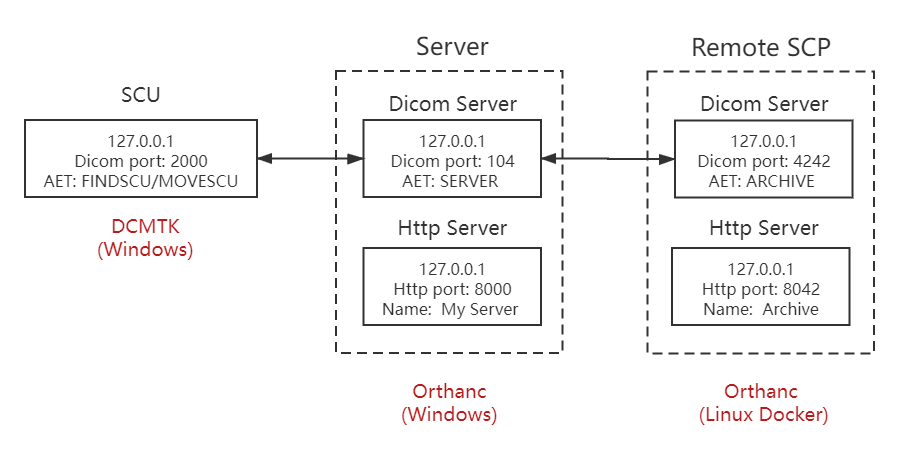
\includegraphics[width=0.8\textwidth]{overview.png}
    \caption{整体系统框图}
    \label{fig:overview}
\end{figure}
\subsection{Server的配置}
根据Orthanc的官方文档\cite{OrthancBook},Orthanc在安装完毕时即提供了默认配置,包括默认的sqlite数据库、默认的Dicom服务、默认的http服务及其端口,因此只需要修改自己需要的部分,其他部分均会由Orthanc读取默认配置文件。本次实验采用的配置文件server\_config.json内容如下:

\begin{lstlisting}[language=C]
    // server_config.json
    {
        "Name": "My Server",
        "HttpPort": 8000,
        "DicomAet": "SERVER",
        "DicomPort": 104,
        "RemoteAccessAllowed" : true,
        "DicomModalities" : {
            "local" : [ "FINDSCU", "127.0.0.1", 2000 ],
            "local2" :[ "MOVESCU", "127.0.0.1", 2000 ],
            "archive": [ "ARCHIVE", "127.0.0.1", 4242 ]   
        }
    }
\end{lstlisting}

Server运行在本地104端口下,同时启动了一个4200端口下的http服务。Dicom网络中的其他几个部分也需要在此处声明用于网络传输的连接。由于使用了自定义的配置文件,因此启动Orthanc时需要指定配置文件路径。因此使用了bat脚本来方便Server的启动。脚本runOrthanc.bat内容如下:
\begin{lstlisting}[language=C]
    "D:\Program Files\Orthanc Server\Orthanc" ./server_config.json --trace
\end{lstlisting}
参数--trace或--verbose可以提供调试时的相关信息,由于需要观察日志,因此将--trace选项打开。

\subsection{SCP的配置}
SCP运行在WSL的Docker环境下,与Server的配置同理,根据官方文档\cite{OrthancBook},采用配置如下:

\begin{lstlisting}[language=C]
    # docker-compose.yaml
    version: '3.1'  # Secrets are only available since this version of Docker Compose
    services:
    orthanc:
        image: jodogne/orthanc-plugins:1.9.7
        command: /run/secrets/  # Path to the configuration files (stored as secrets)
        ports:
        - 4242:4242
        - 8042:8042
        secrets:
        - orthanc.json
        environment:
        - ORTHANC_NAME=HelloWorld
    secrets:
    orthanc.json:
        file: orthanc.json
\end{lstlisting}

\begin{lstlisting}[language=C]
    // orthanc.json
    {
        "Name" : "Archive",
        "RemoteAccessAllowed" : true,
        "DicomAet": "ARCHIVE",
        "DicomModalities" : {
            "server" : ["SERVER","127.0.0.1",104]
        }
    }
\end{lstlisting}
SCP运行在本地4242端口下,同时创建了一个8042端口的http服务。启动时只需要使用命令
\begin{lstlisting}[language=C]
    $ docker-compose up
\end{lstlisting}
即可启动服务。


\subsection{通过Web应用上传Dicom文件}
通过运行上述脚本运行Orthanc Server,此时http Server端口为4200,Dicom Server端口为104。进入浏览器,输入\url{localhost:4200}进入Orthanc界面,点击顶部的Upload菜单即可进入上传界面。

\begin{figure}[H]
    \centering
    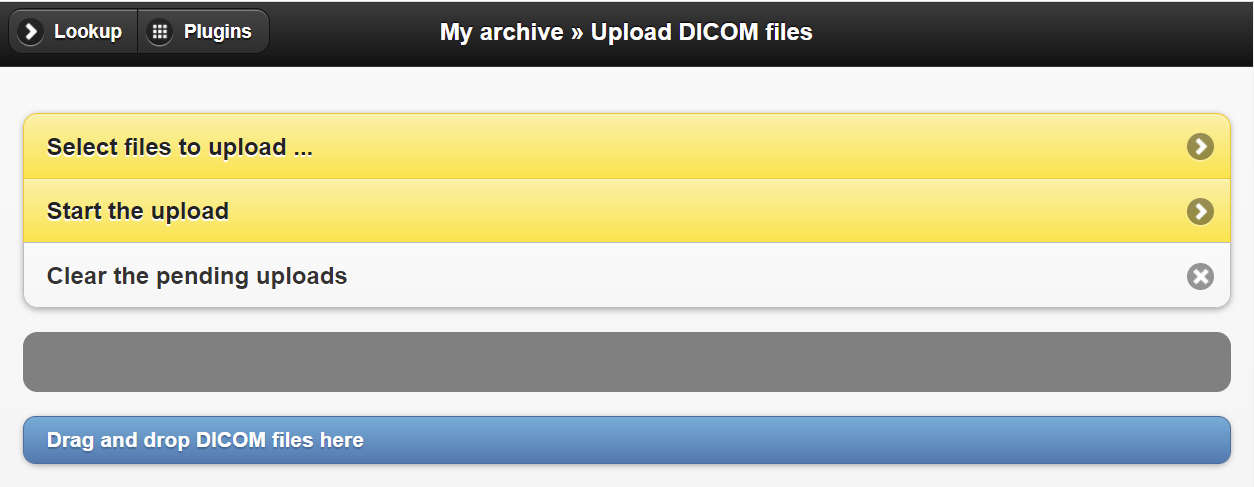
\includegraphics[width=0.6\textwidth]{web upload.png}
    \caption{Orthanc上传界面}
    \label{fig:Orthanc Upload}
\end{figure}

在此界面即可通过拖动和选择文件的方式在图形界面中上传文件。

\subsection{C-STORE的实现}
上述的方式虽然方便,但需要逐个选择上传的文件。如碰到数据量较大的情况就很不方便。此时可以选择通过DCMTK借助命令行脚本的方式上传。

在DCMTK中,C-STORE的命令被封装在storescu.exe中,通过DCMTK官网的文档,我们可以得知其使用方法\cite{DCMTK}:
\begin{lstlisting}[language=C]
    storescu.exe -d -aec ARCHIVE localhost 104 $file
\end{lstlisting}
命令行参数-d输出调试信息,-aec指定应用实体名字,并指定端口号和上传文件。通过PowerShell脚本(storeDCM.ps1)即可批量上传一个文件夹下的所有DCM文件。足够实现一个序列或者检查的批量上传。
\begin{lstlisting}
    $files= Get-ChildItem -Path .\*.dcm 
    foreach($file in $files)
    {
        storescu.exe -d -aec SERVER localhost 104 $file
    }
\end{lstlisting}

\subsection{C-FIND的实现}
同样,C-FIND也只涉及SCU和Server两个应用实体。同样通过DCMTK的官方文档得知,可以使用findscu.exe实现C-FIND功能,具体命令如下:
\begin{lstlisting}
    findscu.exe -ll trace -P localhost 104 
        -k QueryRetrieveLevel=Patient 
        -k PatientID=PID-20210831-161031-1377 
        > ./log/cfind_scu.log
\end{lstlisting}
根据以上条件可以查询到符合指定PatientID的所有Dicom文件。同时指定了trace(最高的输出等级)并将log重定向至cfind\_scu.log文件。

\subsection{C-MOVE的实现}
与C-STORE和C-FIND不同,C-MOVE涉及到三个应用实体,即SCU、本地Server以及模拟的运行在Linux下的远程SCP。同样通过DCMTK的官方文档得知,可以使用movescu.exe实现C-MOVE功能,具体命令如下:
\begin{lstlisting}
    movescu.exe -ll trace -aec SERVER localhost 104 -aem ARCHIVE 
        -k QueryRetrieveLevel=Patient 
        -k PatientID=PID-20210831-161031-1377 
        -k SeriesNumber=8003
        > ./log/cmove_scu.log
\end{lstlisting}
可以将指定PID的指定序列从本地Server拷贝到SCP。同时指定了trace(最高的输出等级)并将log重定向至cmove\_scu.log文件。

\section{log日志内容解析}

\begin{table}[H] 
    \centering  
    \caption{\label{tab:test}缩写和名称对照表}   
    \begin{tabular}{ccc}    
        \toprule    
        缩写 & 全称(英文) & 全称(中文) \\    
        \midrule   
        PDU & Protocol Data Units & 协议数据单元 \\   
        DIMSE & DICOM Message Service Element & DICOM消息服务 \\   
        SOP & Service Object Pair & 服务对象对 \\
        \bottomrule   
    \end{tabular}  
\end{table}

每次运行时,都记录下SCU和SCP的日志,无论从SCU还是SCP来看,每次Dicom网络通信的日志可以分为以下几个部分:
\begin{enumerate}
    \item Associate RQ/AC PDU的交换
    \item DIMSE的发送和接收
\end{enumerate}
而根据每次操作的种类和参数的不同,PDU和DIMSE的内容会有所不同。

第一部分是Associate RQ/AC PDU的交换。这一部分可以分为如下几个步骤:
\begin{enumerate}
    \item SCU生成并发送Associate RQ PDU。
    \item SCP收到Associate RQ PDU后根据状态返回Associate AC PDU(接受连接)或Associate RJ PDU(拒绝连接)。
\end{enumerate}
Associate AC PDU中包含如下信息:
\begin{figure}[H]
    \centering
    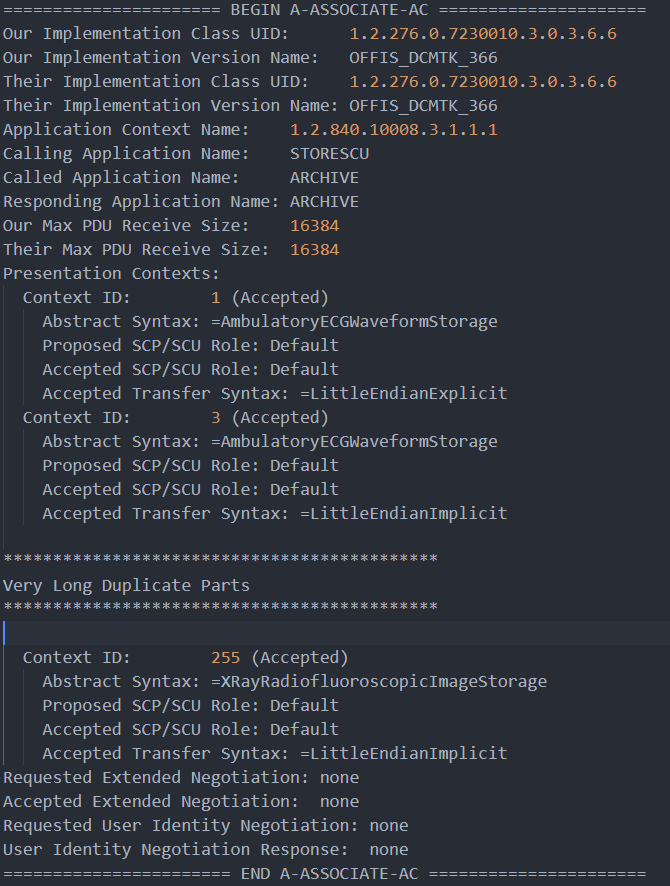
\includegraphics[width=0.5\textwidth]{PDU.png}
    \caption{Associate AC PDU}
    \label{fig: log PDU}
\end{figure}

其中包括协议的class ID,协议实现的版本号,PDU的大小,应用上下文Context等信息。Context共有256段,每段都会返回连接状态(Accepted/Proposed)、Abstract Syntax、SCP/SCU Role等信息。这一部分的信息不包括上传文件的信息,仅供建立连接使用。

第二部分是DIMSE的发送和接收。这一部分可以分为如下几个步骤:
\begin{enumerate}
    \item SCU以OUTGOING DIMSE MESSAGE形式发送一个RQ。
    \item SCP收到INGOING DIMSE MESSAGE后根据状态同样以OUTGOING DIMSE MESSAGE形式发送RSP给SCU。
    \item SCU收到响应后确认状态,整个流程结束。
\end{enumerate}

对于各种操作,Associate RQ/AC PDU和DIMSE交换过程基本类似。不同的是后面的DIMSE的类型和参数不同,因此以下分别对各自的DIMSE内容进行解析。
\subsection{C-STORE DIMSE内容解析}

这一过程中的log显示如下:
\begin{figure}[H]
    \centering
    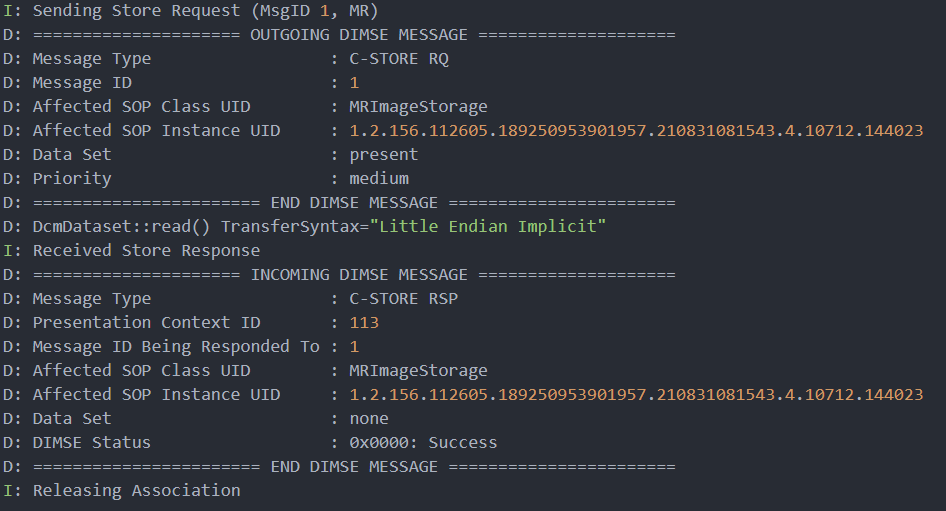
\includegraphics[width=0.6\textwidth]{store_DIMSE_scu.png}
    \caption{C-STORE SCU DIMSE}
\end{figure}

\begin{figure}[H]
    \centering
    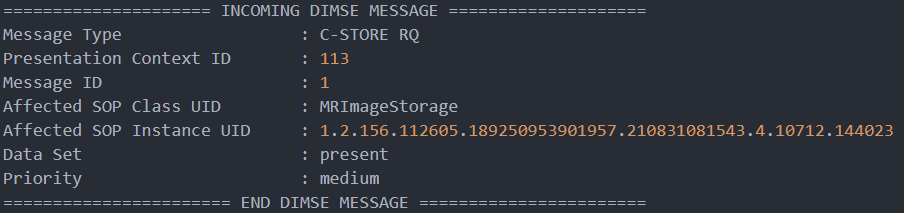
\includegraphics[width=0.6\textwidth]{store_DIMSE_scp.png}
    \caption{C-STORE SCP DIMSE}
\end{figure}
我们可以在其中看到两类DIMSE,RQ和RSP。
C-STORE RQ的内容包括以下几个字段:消息类型、消息ID、SOP的类和实例UID、数据集合消息优先级。
C-STORE RSP的内容包括以下几个字段:消息类型、上下文ID、响应对象的ID、SOP的类和实例UID、数据集和DIMSE状态等信息。

最后DIMSE状态若显示为success,则整个C-STORE流程成功进行。

\subsection{C-FIND DIMSE内容解析}
这一过程中的log显示如下:
\begin{figure}[H]
    \centering
    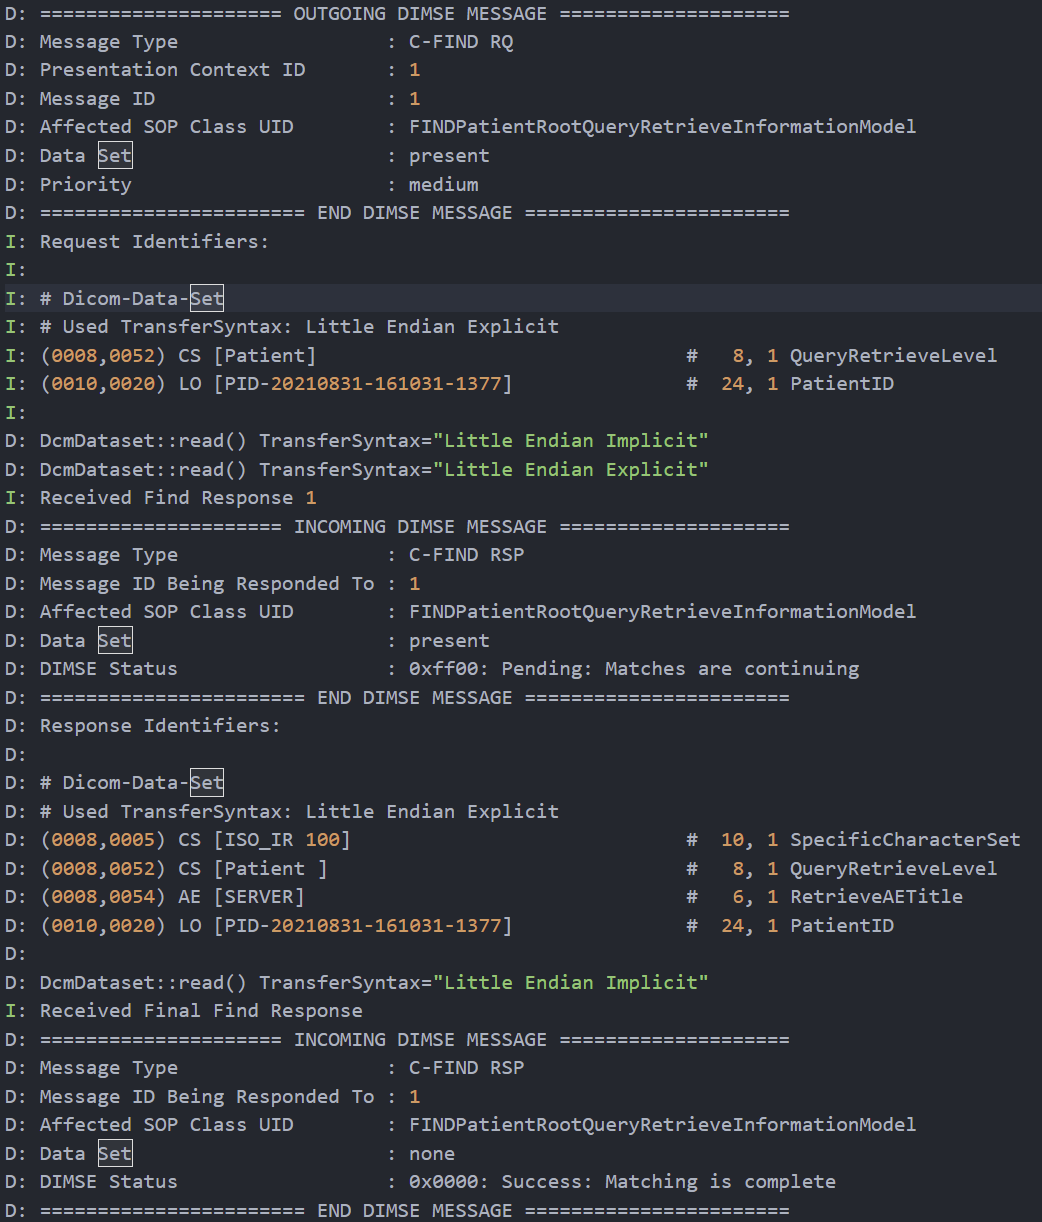
\includegraphics[width=0.6\textwidth]{find_DIMSE_scu.png}
    \caption{C-FIND SCU DIMSE}
\end{figure}

\begin{figure}[H]
    \centering
    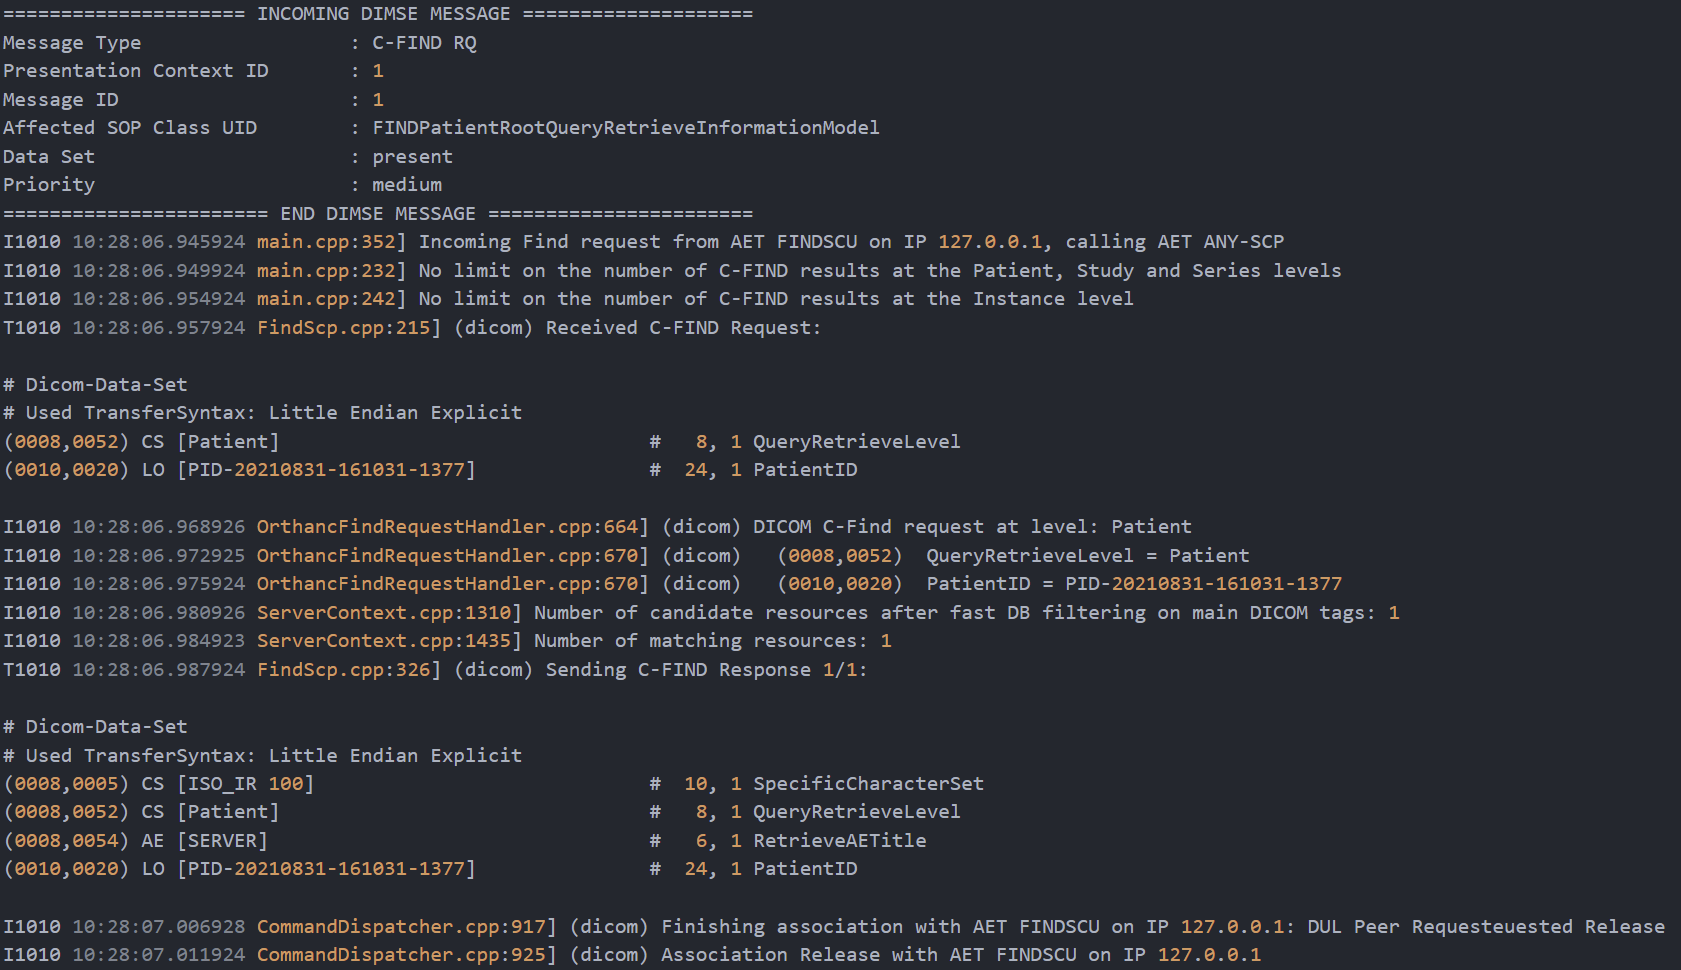
\includegraphics[width=0.6\textwidth]{find_DIMSE_scp.png}
    \caption{C-FIND SCP DIMSE}
\end{figure}
我们可以在其中看到两类DIMSE,RQ和RSP。
C-FIND RQ的内容包括以下几个字段:消息类型、消息ID、SOP的类UID、数据集和消息优先级。其中SOP类分为两种,FINDPatientRootQueryRetrieveInformationModel和FINDStudyRootQueryRetrieveInformationModel,分别对应了DICOM标准中的两种数据获取模型。可以在使用C-FIND时根据需要指定参数切换。
C-FIND RSP的内容包括以下几个字段:消息类型、响应对象的ID、SOP的类和实例UID、数据集和DIMSE状态等信息。当最后DIMSE状态若显示为success,则整个C-STORE流程成功进行。

\subsection{C-MOVE DIMSE内容解析}
对于C-MOVE,情况则有些不同。由于C-MOVE可能涉及多个文件的移动,因此SCU会发送一次RQ,随后根据需要移动的文件数量连续返回若干个RSP。显示的log如下图:
\begin{figure}[H]
    \centering
    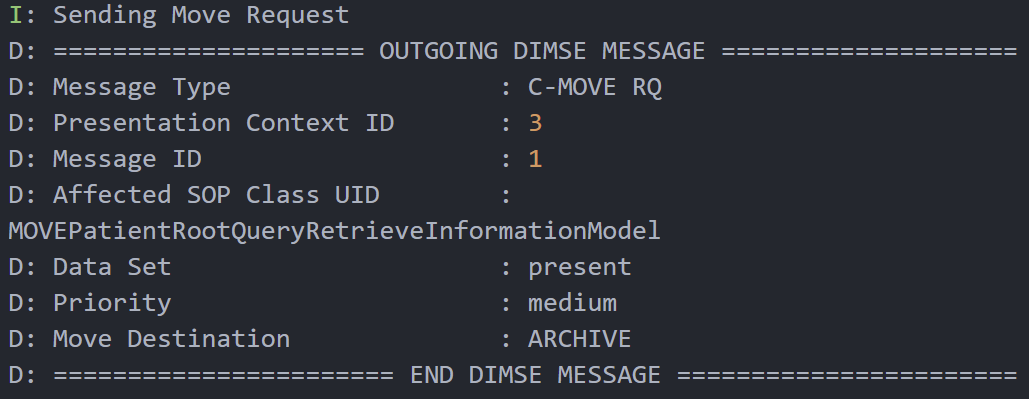
\includegraphics[width=0.6\textwidth]{move_outgoing.png}
    \caption{C-MOVE RQ DIMSE}
\end{figure}

\begin{figure}[H]
    \centering
    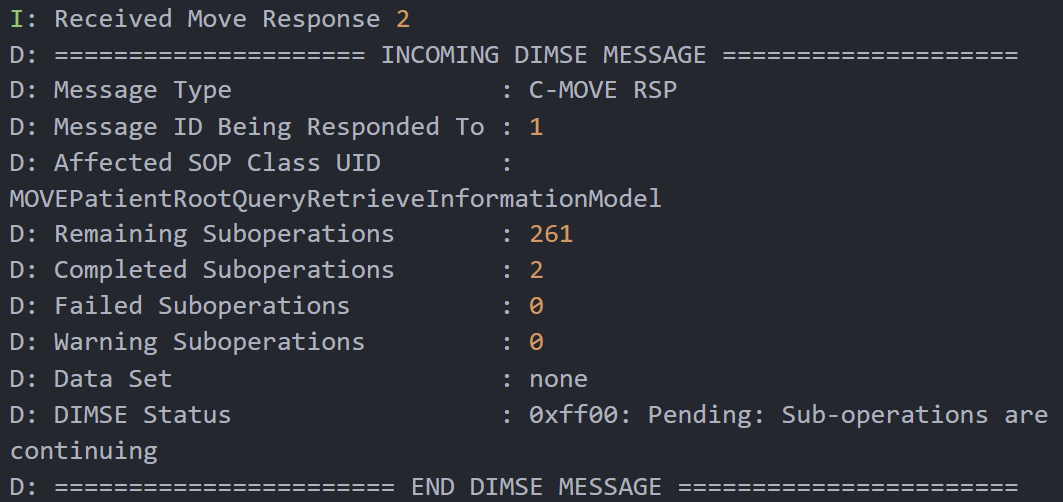
\includegraphics[width=0.6\textwidth]{move_incoming.png}
    \caption{C-MOVE RSP DIMSE}
\end{figure}

其中,RQ只发送一次,内容包括包括以下几个字段:消息类型、消息ID、上下文ID、SOP的类UID、数据集、消息优先级和C-MOVE的目的地。其中SOP类与C-FIND对应分为两种,MOVEPatientRootQueryRetrieveInformationModel和MOVEStudyRootQueryRetrieveInformationModel,分别对应了DICOM标准中的两种数据获取模型。可以在使用C-MOVE时根据需要指定参数切换。

返回的RSP与需要移动的文件数相同,内容包括以下几个字段:消息类型、响应对象的ID、SOP的类UID、剩余、已完成、失败、警告的操作数量、数据集和DIMSE状态等信息。其中DIMSE状态可能包括:Success(全部完成),Sub-operations complete-No failures or warnings(单个文件完成),Sub-operations are continuing(正在移动当前文件)等。当最后传输成功完成时,会返回0x0000: Success: Sub-operations complete - No failures or warnings。

\section{实验感想}

本次实验尝试使用了现有的开源软件搭建了mini-PACS服务器,并尝试了Dicom文件的上传并查看了日志。在实验过程中,遇到过如下几个问题:
\begin{enumerate}
    \item 端口冲突。在调试时,有时会发现Orthanc由于端口冲突无法启动的情况。\\解决方法:在命令行kill掉占用端口的进程或者修改配置文件换用其他端口号。
    \item 在尝试三个AET时,发现Dicom网络通信无法连接。\\ 解决方法:在各自的配置文件中添加所需的AET使其能够相互识别和通信。
\end{enumerate}

本实验所用的脚本和log文件均已附在压缩包中,附上Orthanc下载地址:\url{https://www.orthanc-server.com/download.php}。

\bibliography{references}
\end{document}
